% -*- coding: utf-8 -*-
% Podsumowanie "na chlopski rozum". Kompilacja: pdflatex (dwa przebiegi). Ryciny w fig/.
\documentclass[12pt,a4paper]{article}
\usepackage[utf8]{inputenc}
\usepackage[T1]{fontenc}
\usepackage[polish]{babel}
\usepackage[margin=2.5cm]{geometry}
\usepackage{graphicx}
\usepackage{xcolor}
\usepackage{mdframed}
\usepackage{enumitem}
\usepackage{parskip}
\usepackage[hidelinks]{hyperref}

\definecolor{akcent}{RGB}{0,90,160}
\definecolor{ramka}{RGB}{235,242,250}
\newmdenv[backgroundcolor=ramka,linecolor=akcent,linewidth=0.8pt,
  roundcorner=4pt,skipabove=8pt,skipbelow=8pt,
  innertopmargin=8pt,innerbottommargin=8pt]{infobox}
\newcommand{\waz}[1]{\textcolor{akcent}{\textbf{#1}}}
\setlist{itemsep=2pt,topsep=3pt}

\title{\vspace{-1.5cm}\textbf{Predykcja zapchania młyna węglowego}\\[2pt]
\large Podsumowanie „na chłopski rozum"}
\author{}
\date{}

\begin{document}
\maketitle
\vspace{-1.2cm}

\begin{infobox}
\textbf{O co chodzi w jednym zdaniu:} uczymy komputer, żeby \waz{z wyprzedzeniem
ostrzegał}, że młyn mielący węgiel zaraz się zapcha --- zanim trzeba będzie go
awaryjnie odstawić. Trochę jak czujnik, który mówi „za pół godziny będzie korek",
a nie dopiero „stoisz w korku".
\end{infobox}

\section*{1. Co to w ogóle jest młyn i co znaczy „zapchanie"}

W elektrociepłowni węgla nie wrzuca się do kotła w kawałkach --- najpierw trzeba
go zemleć na drobny pył, żeby ładnie się palił. Robi to \waz{młyn węglowy}
(tu: cztery sztuki, nazwane MW1, MW2, MW3, MW4). Młyn jednocześnie mieli węgiel
i \waz{dmucha} go gorącym powietrzem do kotła --- powietrze niesie pył jak wiatr
niesie kurz.

\waz{Zapchanie (dławienie)} to sytuacja, gdy w młynie zbiera się za dużo węgla
i powietrze przestaje go przepychać. Wyobraź sobie \waz{odkurzacz, który wciągnął
za dużo} --- silnik wyje, a ssie coraz słabiej. Z młynem jest podobnie: pracuje
coraz ciężej, a „przewiew" spada. Jak się to zignoruje, młyn trzeba awaryjnie
wyłączyć, co kosztuje i destabilizuje pracę bloku.

\section*{2. Skąd wiemy, co się dzieje w młynie}

Z młyna co minutę spływa kilkadziesiąt pomiarów (moc silnika, ile węgla podajemy,
jak mocno dmuchamy, jaka jest temperatura itd.). Mamy taki zapis za \waz{cały luty
2026}. To są nasze „dane" --- surowy dziennik pracy maszyny minuta po minucie.

\begin{infobox}
\textbf{Mały haczyk:} w danych był bałagan (różne zapisy daty w jednym pliku, dziwne
kodowanie polskich znaków, dziury w pomiarach). Pierwsza robota to było
\waz{posprzątanie} tego tak, żeby dało się w ogóle policzyć cokolwiek sensownego.
\end{infobox}

\section*{3. Jak rozpoznajemy, że młyn się dławi (objawy)}

Okazało się, że zapchanie zawsze wygląda \waz{tak samo} i rozwija się powoli ---
i to jest dobra wiadomość, bo coś powtarzalnego da się przewidzieć. Kolejność objawów:

\begin{enumerate}
  \item automat „dodaje gazu" wentylacji \waz{aż do maksimum} (100\%, nie ma już zapasu),
  \item mimo to \waz{przewiew i tak spada} --- znak, że coś zapycha drogę powietrzu,
  \item \waz{silnik młyna bierze coraz więcej mocy} (jak ten przeciążony odkurzacz),
  \item w końcu automatyka \waz{awaryjnie przykręca dopływ węgla}, młyn się „przeczyszcza".
\end{enumerate}

Najważniejsze: te objawy widać \waz{na 1--2 godziny przed} kulminacją. Jest więc czas,
żeby zareagować.

\begin{figure}[h]
\centering
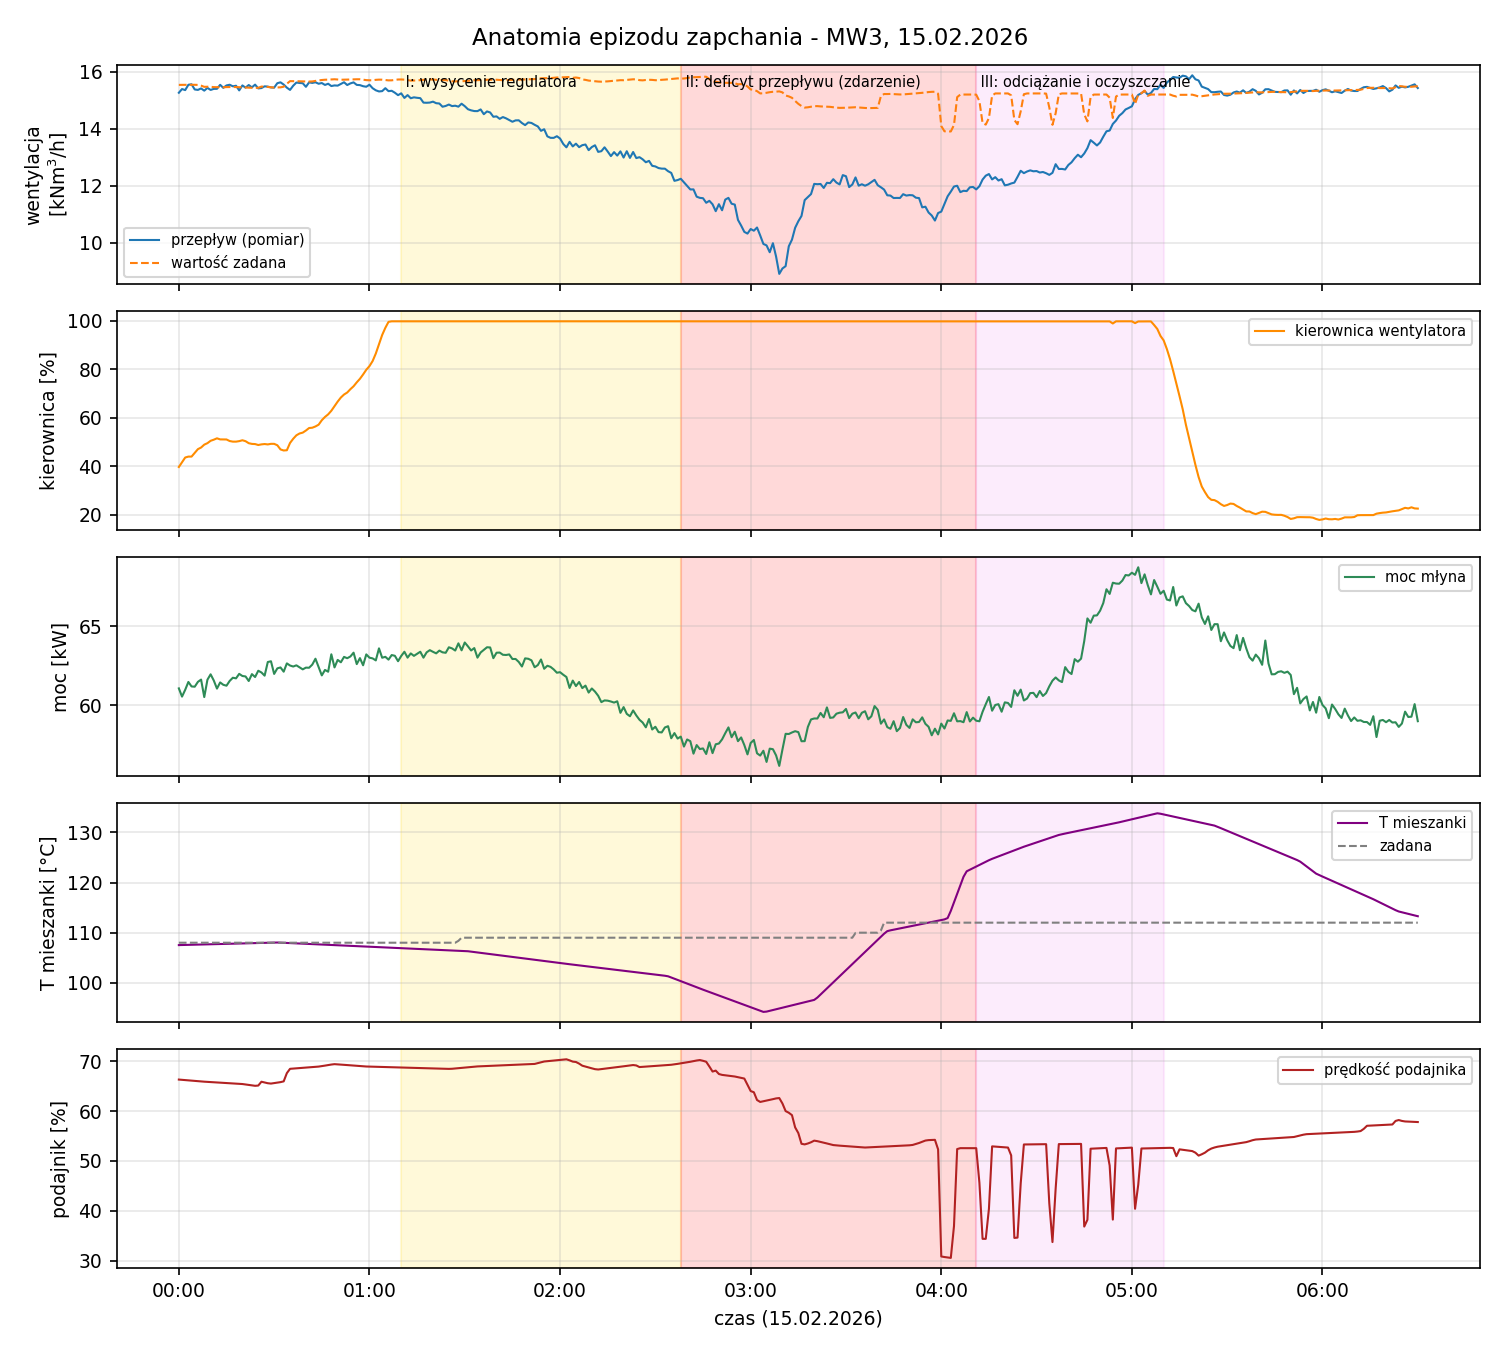
\includegraphics[width=0.82\textwidth]{fig/anatomia_zdarzenia.png}
\caption*{\small Tak wygląda jeden epizod w danych: na górze przewiew (spada),
poniżej moc młyna (rośnie). Widać, że to nie nagły skok, tylko \waz{narastający problem}.}
\end{figure}

\section*{4. Jak nauczyliśmy komputer ostrzegać}

Tu nie ma żadnej magii. Robota w dwóch krokach:

\textbf{Krok A --- liczymy „wskaźniki zdrowia".} Z surowych pomiarów liczymy kilka
mówiących liczb, np.:
\begin{itemize}
  \item \waz{deficyt} --- o ile faktyczny przewiew jest słabszy, niż być powinien
        (im większy, tym gorzej),
  \item \waz{drożność} --- czy przy danym „gazie" powietrze w ogóle leci
        (jak sprawdzenie, czy rura nie jest zatkana),
  \item \waz{ile mocy idzie na zmielenie tej samej porcji węgla} (rośnie, gdy się zapycha).
\end{itemize}
W sumie takich wskaźników jest 39 i --- co ważne --- liczone są \waz{tylko z przeszłości},
żeby model nie „podglądał przyszłości" i nie oszukiwał.

\textbf{Krok B --- model przewidujący.} Te wskaźniki podajemy programowi
(\waz{LightGBM} --- to taki sprytny „kalkulator reguł", który sam się uczy na
przykładach, jakie kombinacje wartości zwiastują kłopoty). Na wyjściu daje
\waz{wynik od 0 do 1} --- czyli „jak bardzo pachnie zapchaniem". Gdy wynik jest
wysoko przez \waz{3 minuty z rzędu}, podnosimy alarm. Trzy minuty zamiast jednej ---
żeby nie wyć przy każdym przypadkowym drgnięciu.

\begin{infobox}
\textbf{Dlaczego nie „sztuczna inteligencja" jak ChatGPT / sieci neuronowe?}
Bo do nauczenia takich dużych modeli trzeba \waz{mnóstwa przykładów}, a my mamy
tylko \waz{5 zapchań} z jednego miesiąca. Przy tak małej liczbie przykładów prosty,
przejrzysty model jest \waz{pewniejszy} i można sprawdzić, „dlaczego" tak zdecydował.
Sieci neuronowe też przetestowaliśmy --- wyszły gorzej i niestabilnie.
\end{infobox}

\section*{5. Co z tego wyszło (wyniki po ludzku)}

\begin{infobox}
\textbf{Najważniejsze: model złapał \waz{wszystkie 5 z 5} prawdziwych zapchań,
średnio \waz{30 minut wcześniej}, prawie nie podnosząc fałszywych alarmów}
(mniej więcej \waz{1 fałszywka na ~17 dni} pracy jednego młyna). Wersja
łączona (model + prosta reguła fizyczna jako drugi strażnik) ostrzegała jeszcze
wcześniej --- średnio \waz{około 51 minut przed}.
\end{infobox}

Mówiąc wprost: gdyby to działało na żywo, operator dostawałby sygnał „uważaj na MW3,
za jakieś pół godziny zacznie się dławić" --- z czasem na spokojną reakcję, a nie
gaszenie pożaru.

Dodatkowo, od strony „inżynierskiej" potwierdziliśmy fizykę: tuż przed zapchaniem
\waz{drożność spada dramatycznie} (na jednym młynie aż o 83\%) --- czyli liczby
zgadzają się z tym, co podpowiada zdrowy rozsądek.

\section*{6. Czy to już działa? Uczciwie}

To jest \waz{obiecujący prototyp (dowód, że się da)} --- a nie gotowy produkt.
Dlaczego warto zachować ostrożność:
\begin{itemize}
  \item mamy tylko \waz{5 zapchań z jednego miesiąca} --- za mało, żeby mieć pewność,
        że model poradzi sobie zawsze (inny węgiel, inna pora roku mogą wyglądać inaczej);
  \item \waz{nie mieliśmy oficjalnego dziennika awarii} --- sami „wyznaczyliśmy", co jest
        zapchaniem, na podstawie objawów; warto to potwierdzić z obsługą bloku;
  \item żeby zaufać temu na poważnie, trzeba \waz{6--12 miesięcy danych} i testów na żywo.
\end{itemize}

\section*{Słowniczek (5 słów)}
\begin{description}[leftmargin=2.2cm,style=nextline,itemsep=2pt]
  \item[Młyn (MW1--4)] maszyna mieląca węgiel na pył i wdmuchująca go do kotła.
  \item[Zapchanie] nadmiar węgla dławi przepływ powietrza --- młyn „się krztusi".
  \item[Cecha/wskaźnik] mówiąca liczba policzona z pomiarów (np. deficyt, drożność).
  \item[Model] program, który z tych wskaźników typuje ryzyko zapchania (0--1).
  \item[Wyprzedzenie] o ile minut wcześniej padł alarm przed faktycznym zapchaniem.
\end{description}

\end{document}
